\subsection{Einführung}
\subsubsection{Netze}
\begin{itemize}
\item A-Netz (1958 - 1976)
\begin{itemize}
\item Handvermittlung
\item sehr teure Endgeräte
\item Kapazitätsgrenzen (Rufnummerngrenzen)
\item Höchstteilnehmerzahl 11000(1971)
\end{itemize}
\item B/B2-Netz(1972-1994)
\begin{itemize}
\item Selbstwahl ab 1977 Übernahme von A-Frequenzen durch
\item B2-Netz
\item keine einheitliche Vorwahl(genauer Standort musst bekannt sein)
\item Höchstteilnehmerzahl 27000 (1986)
\end{itemize}
\item C-Netz (1985-)
\begin{itemize}
\item Analoges Mobilfunknetz
\item Selbstwahl mit Handover
\item Einheitliche Vorwahl 0161
\item Dienste
\end{itemize}
\item D-Netz
\begin{itemize}
\item Ziel war neues Netz
\begin{itemize}
\item Subjektiv gute Sprachqualität
\item Hohe Sicherheit
\item Preisgünstige Endgeräte, niedrige Betriebskosten
\item Internationales Roaming
\item Unterstütung von Handgeräten
\item Unterstützung neuartiger Dienste
\item ISDN Kompabilität
\item 1989 wurd die Verantwortung für GSM an das ETSI übertragen, 1990 wurden Spezifikationen publiziert
\end{itemize}
\item 1990 Abschluss der Standardisierung 
\item 1992 Kommerzieller Start des ersten GSM Netztes (T-D1)
\item 1993 Neudefinition für GSM (SAM 900,1800 und 1900(USA))
\item 1995 Weltweit 120 GSM-Netze 
\item 1998 Über 200 GSM-Netzbetreiber in über 110 Ländern
\end{itemize}
\end{itemize}

\subsection{Netzstruktur und Aufbau}
\begin{itemize}
\item Multiplexing
\begin{itemize}
\item Raummultiplex - Netzstruktur und Aufbau
\item Frequenzmultiplex - Frequenzplan
\item Zeitmultiplex - Rahmenstruktur und Kanalplanung
\end{itemize}
\item Übertragungsprobleme
\begin{itemize}
\item Bitfehlerrate - Kanalcodierung
\item Rayliegh Fading - Frequenzy Hopping
\item Time Dispersion - Adaptive Equalization
\item Rahmensynchronisation - Timing Advance
\end{itemize}
\item Architektur
\begin{itemize}
\item Kanalstruktur
\item Protokollstack
\end{itemize}
\item Verhalten
\begin{itemize}
\item Anmelden, Abmelden
\item Sicherheitsprotokoll
\item Verbindungsauf- und abbbau
\item Verbindungssteuerung
\end{itemize}
\end{itemize}

\subsection{Multiplextechnik}
\subsubsection{Raummultiplex durch Zellen}
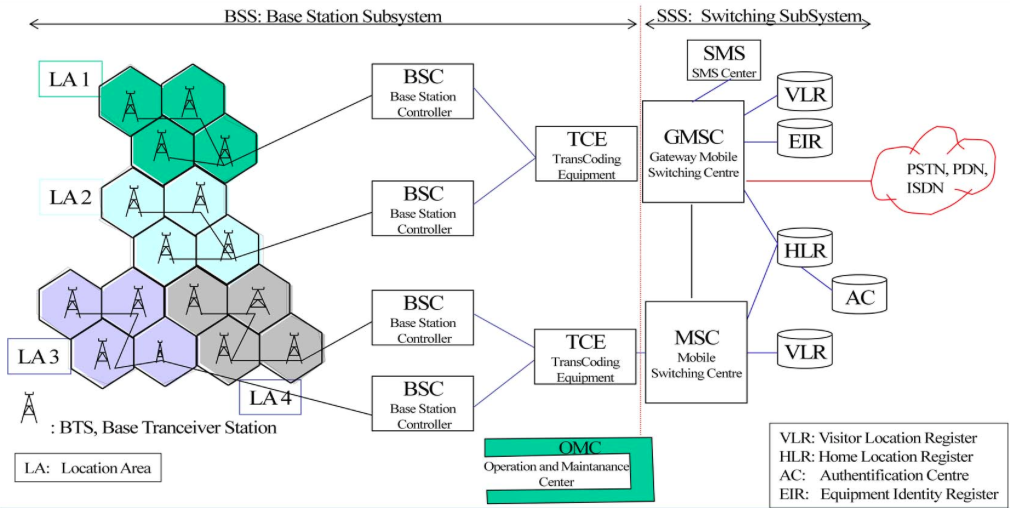
\includegraphics[width = \linewidth]{./Pics/GSMZellen}

\begin{itemize}
\item Wiederverwendung der Frequenz
\item Unterschiedliche Zelltypen
\begin{itemize}
\item Macro Cell
\item Micro Cell
\item Pico Cell
\item Femto Cell
\item Sectorized Cell
\item Umbrella Cell
\item Extended Cell
\end{itemize}
\item Einsatz der Zelltypen verkehrsabhängig, siehe auch Verlustsysteme und Grade of Service (GOS)
\item für die Planung wird pro Zelle ein Verkehr von 25 - 35 mErlang und ein GOS von 2\% veranschlagt
\end{itemize}
\vspace{0.5 cm}
\begin{minipage}{0.7 \linewidth}
\begin{itemize}
\item Pico-Zelle
\begin{itemize}
\item Maximale Reichweite 100m
\item Inhouse sowie Gebäude- und Grundstückversorgung
\end{itemize}
\item Micro-Zelle
\begin{itemize}
\item Reichweite 100m bis 2 km
\item Hohes Verkehrsaufkommen
\end{itemize}
\item Macro-Zelle
\begin{itemize}
\item Reichweite 2 km bis 35 km
\item Schnelle Abdeckung grosser Gebiete 
\item Gernges Verkehrsaufkommen
\item Verwendung als Schirm über Micro-Zellen
\end{itemize}
\item Sektorisierte Zelle
\begin{itemize}
\item Ein Aufbauort (site) zur Realisierung der Sektorzellen
\item Hier werden mehrere BTS zusammengestellt
\item Dienen zur Abdeckung von Gebieten mit hohem erwartetem Verkehrsaufkommen
\end{itemize}
\end{itemize}
\end{minipage}
\begin{minipage}{0.3 \linewidth}
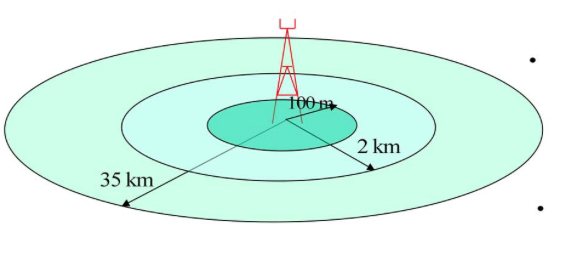
\includegraphics[width = \linewidth]{./Pics/GSMZellen2}
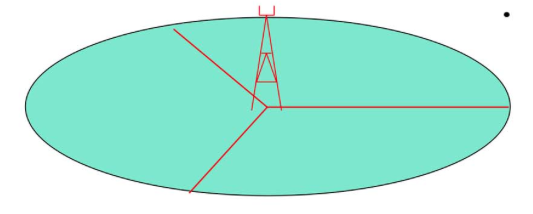
\includegraphics[width = \linewidth]{./Pics/GSMZellen3}
\end{minipage}
\begin{minipage}{0.5 \linewidth}
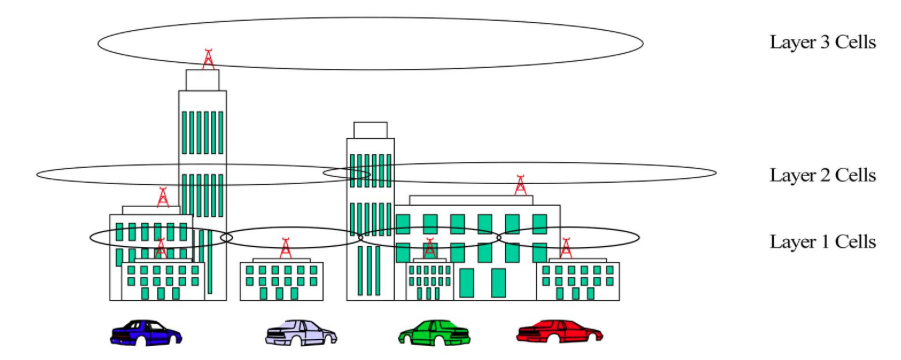
\includegraphics[width = \linewidth]{./Pics/GSMZellenPrinzip}
\end{minipage}
\begin{minipage}{0.5 \linewidth}
\begin{itemize}
\item Die Zellen werden nach Bewegungsgeschwindigkeit des User gewählt
\item So können unnötig viele Zellenwechsel verhindert werden
\item In Ballungsgebieten, in denen sich viele User auf kleinem Raum befinden und nicht grossartig Bewegen, kann man Layer 1 Zellen mehr Bandbreite zu Verfügung stellen
\end{itemize}
\end{minipage}

\subsubsection{Frequenzmultiplex}
\begin{minipage}{0.5 \linewidth}
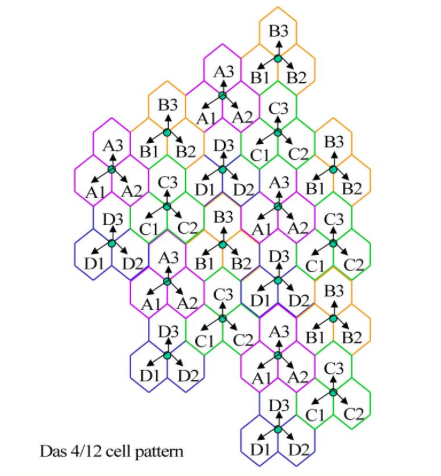
\includegraphics[width = \linewidth]{./Pics/GSMFrequenzplan}
\end{minipage}
\begin{minipage}{0.5 \linewidth}
\begin{itemize}
\item Gruppen von Frequenzen werden zu so genannten Clustern zusammengefasst
\item Aus Interferenz-gründen ist der Abstand zwischen wieder benutzten Frequenzen so gross wie möglich zu halten. Durch Clustering wird dies einfach realisiert
\item Für GSM werden die 3/9 oder 4/12 Re-Use-Pattern empfohlen
\end{itemize}
\end{minipage}
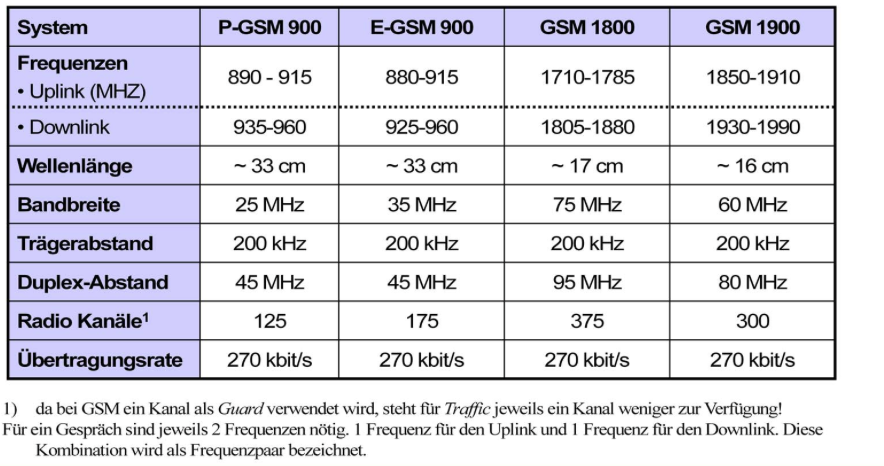
\includegraphics[width = 0.5 \linewidth]{./Pics/GSMFrequenzkonzept}

\subsubsection{Zeitmultiplex}

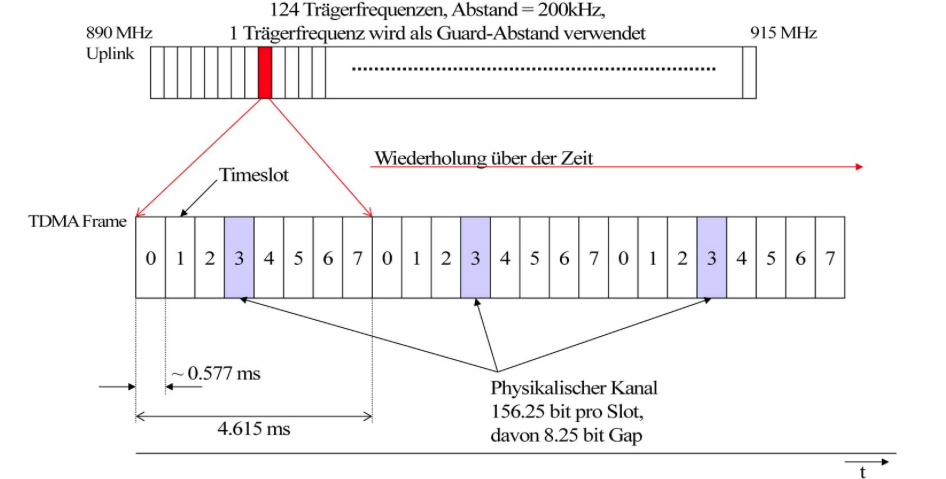
\includegraphics[width = 0.5 \linewidth]{./Pics/GSMRahmenstruktur}

\subsubsection{Mulitplextechniken Überblick}
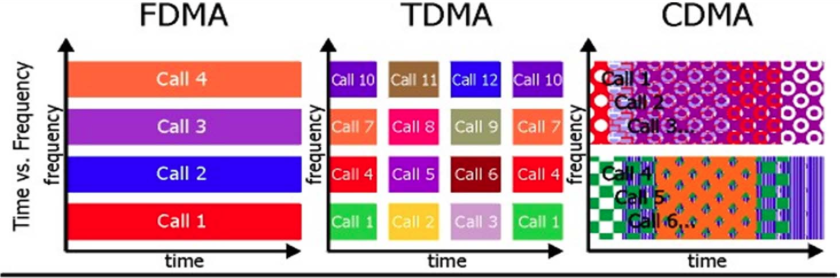
\includegraphics[width = 0.5 \linewidth]{./Pics/GSMMuxTechniken}

\begin{description}
	\item[FDMA] Frequency Division Multiple Access
	\begin{itemize}
		\item Verschieden Frequenzkanäle
		\item Pro Frequenz nur einer der Spricht
	\end{itemize}
	\item[TDMA] Time Division Muliple Access
	\begin{itemize}
		\item Verschieden Frequenzkanäle
		\item Mehrere Timeslots pro Frequenz
		\item Die Übertragungsrate wird auf mehrere Aufgeteilt
	\end{itemize}
	\item[CDMA] Code Division Multiple Access
	\begin{itemize}
		\item Verschieden Frequenzkanäle
		\item Jeder Spricht in einem eigenen Code gleichzeitig
		\item kann man sich anhand mehrere Leute in einem Raum die verschiedene Spachen sprechen vorstellen
	\end{itemize}
\end{description}

\subsection{Übertragungsprobleme}
\begin{minipage}{0.5 \linewidth}
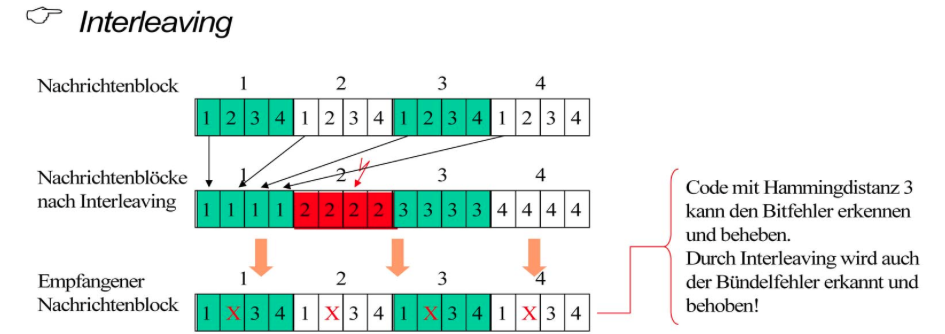
\includegraphics[width = \linewidth]{./Pics/GSMInterleaving}
\end{minipage}
\begin{minipage}{0.5 \linewidth}
\begin{itemize}
\item \textbf{Interleaving}
\item Auftretende Fehler sind meist Bündelfehler, d.h. ein ganzer Burst ist gestört
\item Es ist nicht möglich Codes mit mehr Kontrollstellen einzuführen, um so mehr Fehlerstellen zu korrigieren
\end{itemize}
\end{minipage}


\begin{minipage}{0.5 \linewidth}
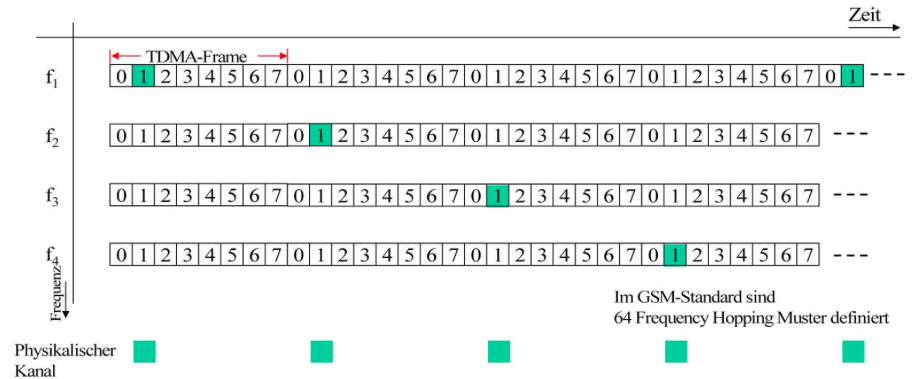
\includegraphics[width = \linewidth]{./Pics/GSMFreqHopping}
\end{minipage}
\begin{minipage}{0.5 \linewidth}
\begin{itemize}
\item \textbf{Rayleigh Fading} ist frequenzabhängig
\item Um bessere Übertragungsqualität zu erreichen, ist eine Bandspreiung sinnvoll
\item Durch \texttt{Frequency Hopping} wird eine Bandspreizung erreicht!
\end{itemize}
\end{minipage}

\subsubsection{Time Dispersion} 

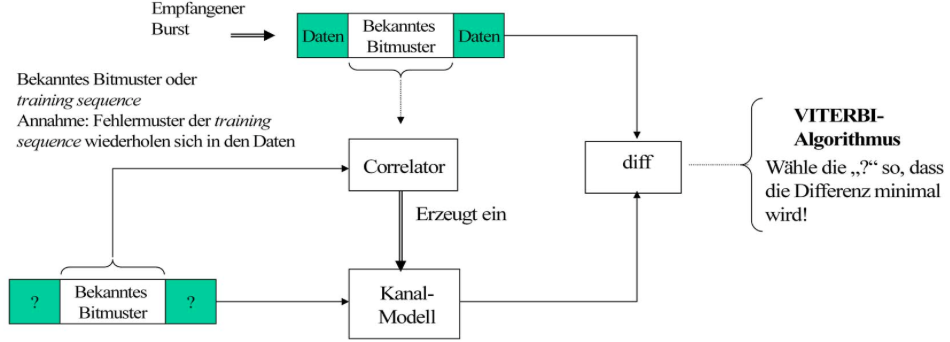
\includegraphics[width = 0.6\linewidth]{./Pics/GSMTimeDispersion}

\subsubsection{Rahmensynchronisation - Timing Advance}
\begin{itemize}
\item Timing Advance ist ein Lösungsansatz der speziell die Rahmensynchronisation vornimmt
\item Hierzu wird ein Protokoll definiert
\begin{itemize}
\item Messen der Laufzeit zwischen MS und BTS
\item Senden einer Korrekturzeit von der BSC via BTS an die MS, ob die MS früher oder später senden muss
\end{itemize}
\item Für die Anmeldeprozedur muss ein verkürzter Burst zur Verfügung gestellt werden
\end{itemize}

\subsubsection{Access Burst}
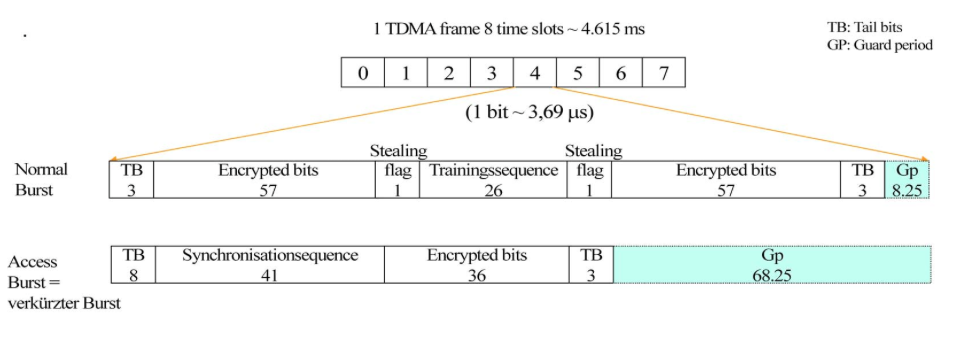
\includegraphics[width = 0.6\linewidth]{./Pics/GSMAccessBurst}

\subsection{Zusammenfassung GSM Übertragungsprozess}

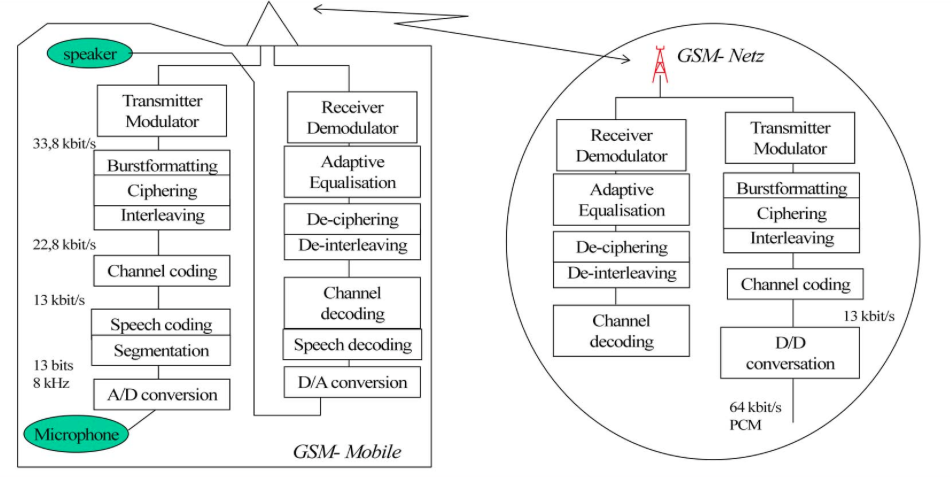
\includegraphics[width = 0.6\linewidth]{./Pics/GSMZusammenfassung}

\subsection{GSM Protokoll Stack}
\begin{minipage}{0.5 \linewidth}
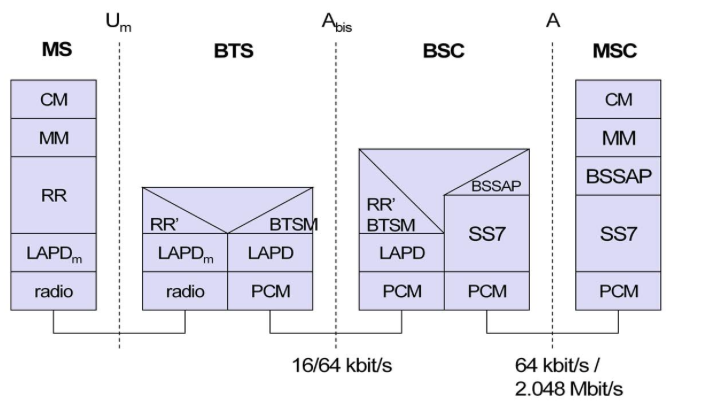
\includegraphics[width = \linewidth]{./Pics/GSMProtokollStack}
\end{minipage}
\begin{minipage}{0.5 \linewidth}
\begin{description}
\item[CM] Communication Management
\item[MM] Mobility Management
\item[RR] Radio Resource Management
\item[LAPD] Link Access Protocol for D-Channel
\item[BTSM] BTS Management
\item[BSSAP] Base Station System Application Part
\item[SS7] Signaling System No. 7
\end{description}
\end{minipage}

\subsection{Kanalstruktur}
\subsubsection{Übersicht}
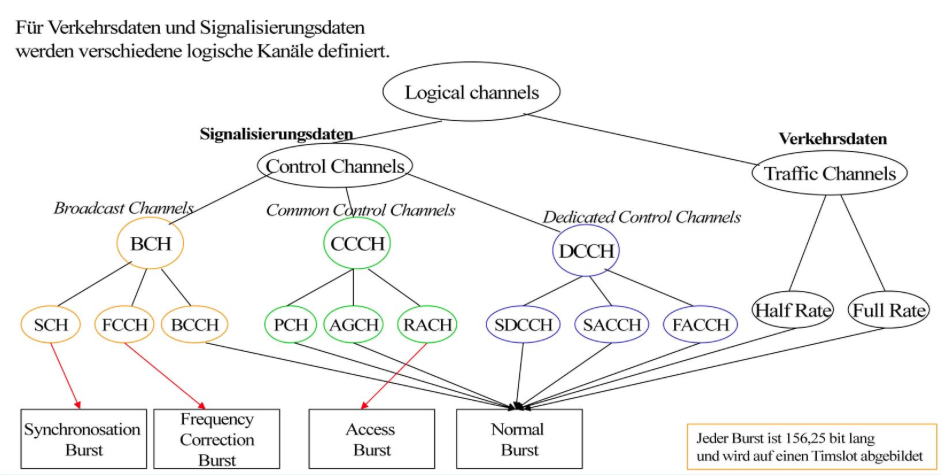
\includegraphics[width = 0.5 \linewidth]{./Pics/GSMKanalstruktur}

\subsubsection{Traffic Channels}
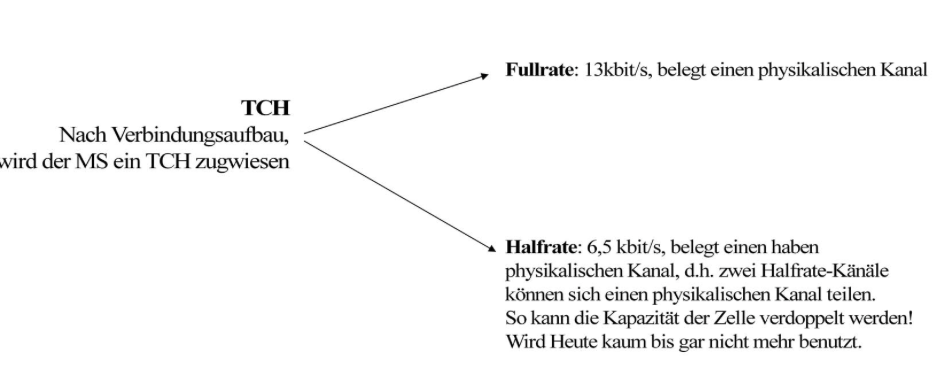
\includegraphics[width = 0.5 \linewidth]{./Pics/GSMTCH}
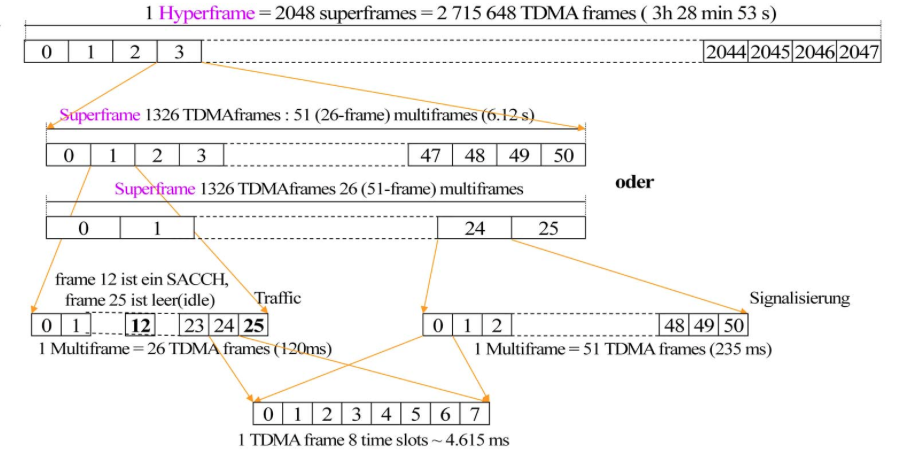
\includegraphics[width = 0.5 \linewidth]{./Pics/GSMFRrameBurstStruktur} $\;$\\ \\
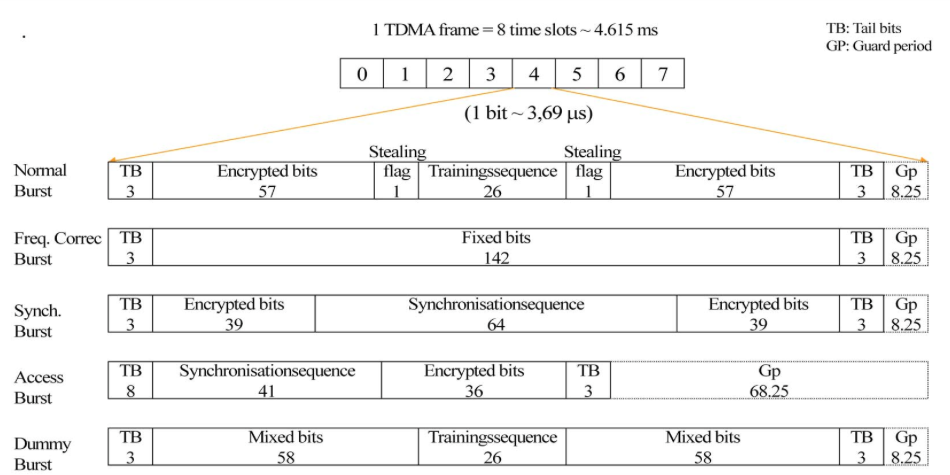
\includegraphics[width = 0.5 \linewidth]{./Pics/GSMBurstStruktur}
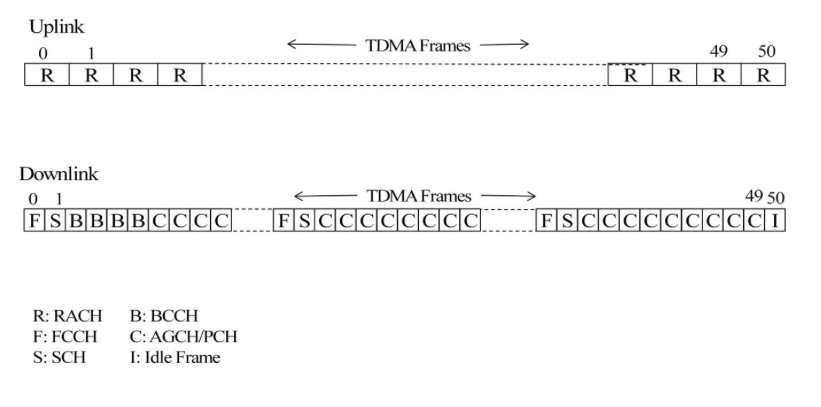
\includegraphics[width = 0.5 \linewidth]{./Pics/GSMMultiframe}
\subsubsection{Signalisierungsdaten}
\begin{tabular}{p{0.15 \linewidth} p{0.15 \linewidth} p{0.3 \linewidth} p{0.3 \linewidth}}
\toprule
Logischer Kanal & Richtung & BTS & MS \\
\midrule
AGCH & Downlink point to point & Weist der MS einen Signalisierungskanal (SDCCH) zu & Empfängt eine Signalisierungskanalzuweisung \\
\midrule
BCCH - Broadcast Control Channel & Downlink point to Multipoint & Verteilt allgemeine Zellinformationen, wie z.B. LAI (Local Area Identity), die BCCH Träger der Nachbarzellen, Max. Ausgangsleistung & Empfängt die LAI und leitet  ggf. ein Location update ein. 
Stellt die Ausgangsleistung ein.
 Erstellt eine List der Nachbarzell-BCCHs für die Leistungsmessungen der BCCH-Träger \\
\midrule
CBCH - Cell Broadcast Channel & Downlink point to multipoint & Dient zum versenden von Broadcast-Kurznachrichten & Empfang von Broadcast-Kurznachrichten\\
\midrule
FACCH Fast Associated Control Channel & Up- und Downlink point to point & Übermittelt Handover-Informationen & Übermittelt Handover-respons\\
\midrule
FCCH - Frequency Correction Channel & Downlink point to Multipoint & Überträgt die Trägerfrequenz & Identifiziert den BCC-Träger und synchronisiert auf der Frequenz \\
\midrule
PCH - Paging Channel & Downlink point to point & Signalisisert einen eingehenden Ruf oder ein SMS. Die Nachricht enthält die Identifikationsnummer des Mobilfunkkunden (IMSI) & Die MS hört regelmässig auf den PCH und reagiert, wenn die eigene Mobile Subscriber ID addressiert wird \\
\midrule
RACH - Random Access Channel & Uplink point to point & Empfängt die Anforderung einer MS einen Signalisierungskanal aufzubauen (SDCCH) & Eigentsändiger Verbindungsaufbau oder Antwort auf Request über den PCH \\
\midrule
SACCH Slow Associated Conrtol Channel & Up- und Downlink point to point & Erteilt Befehle zur Regelung der Sendeleistung und zum timing advance & Sendet durchschnittsmessungen der eigenen BTS (Signalstärke und Qualität) und der Nachbar BTSen (Signalstärke) \\
\midrule
SCH - Synchronisation Channel & Downlink point to Multipoint & Enthält Daten über die TDMA Rahmenstruktur in einer Zelle sowie die BTS - ID & Synchronisiert mit der Rahmenstruktur \\
\midrule
SDCCH - Standalone Dedicated Control Channel & Up- und Downlink point to point & Die BTS schaltet auf einen SDCCH.
Die Verbindungsaufbau Prozedur wird abgewickelt und ein TCH wird zugewiesen.
SDCCH wird auch zur Übermittlung von SMS verwendet & Die MS schaltet auf ein SDCCH.
Die Verbindungsaufbau-Prozedur wird abgewickelt und ein TCH wird zugewiesen (Träger und Slot).\\
\bottomrule

\end{tabular}

\subsection{MSISDN - Mobil Station/Subscriber Integrated Services Digital Network}

\begin{minipage}{0.6 \linewidth}
\begin{itemize}
\item Ordnet Mobiltelefonen eindeutige Nummern zu (Telefonnummer)
\item Die maximale Lände einer MSISDN beträgt 15 digits
\item ist die einzige Nummer, die der Subscriber kennt
\end{itemize}
\end{minipage}
\begin{minipage}{0.4 \linewidth}
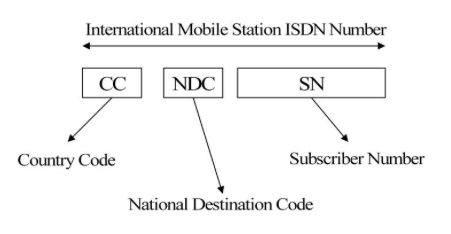
\includegraphics[width =  \linewidth]{./Pics/GSMMSISDN}
\end{minipage}

\begin{minipage}{0.6 \linewidth}
\begin{itemize}
\item IMSI - International Mobile Subscriber Identity
\begin{itemize}
\item Ist die eindeutige Identifikation eines Mobilfunk-Subscribers
\item Alle, zu einem Benutzer gehörenden Informationen, sind unter der IMSI zugreifbar. Ost quasi der Primary key vom HLR
\item Wird benutzt zur Signalisierung innerhalb des PLMN (Public Land Mobile Network)
\item Die IMSI ist gespeichert in der
\begin{itemize}
\item SIM Karte 
\item HLR
\item Serving VLR
\end{itemize}
\end{itemize}
\item TMSI - Temporary Mobile Subscriber Identity 
\begin{itemize}
\item Ist eine temporäre IMSI, die der MS während des Verbindungsaufbaus übergeben wird
\item Soll die Subscriberidentität an der Luftschnittstelle verschleiern
\item Die TMSI
\begin{itemize}
\item hat nur lokale Bedeutung (MSC/VLR Bereich)
\item Nicht grösser als 8 digits
\end{itemize}
\item Die TMSI ändert sich
\begin{itemize}
\item In bestimmten Intervallen
\item Bei einem Ereignis wie z.b. location update
\end{itemize}
\end{itemize}
\item MSRN - Mobile Station Roaming Number
\begin{itemize}
\item ist eine temporäre Nummer (gleicher Aufbau wie MSISDN), due während des Verbindungsaufbaus zu einem Subscriber in ein Netz vergen wird. Die MSRN wird durch das VLR vergeben und ist ebenfalls im HLR abgespeichert
\end{itemize}
\item LAI - Location Area Identity
\begin{itemize}
\item jede LA ist eindeutig durch eine LAI identifizierbar. Wird verwendet für:
\begin{itemize}
\item Paging
\item Location Updating
\end{itemize}
\item LAC - Location Area Code ein 16 Bit-feld zur Identifizierung verschiedener Location Areas in einem PLMN
\end{itemize}
\item CGI - Cell Global Identity
\begin{itemize}
\item Wird zur Identifizierung einer Zelle in einer Location Area benutzt
\end{itemize}
\item BSIC - Base Station Identity Code
\begin{itemize}
\item Dient den Mobilstationen zur Unterscheidung zwischen den benachbarten Basisstationen
\item besteht aus NCC (Network Color Code, 3 Bit) zur Identifizierung des PLMN und 
\item BCC (Basestation Color Code, 3 Bit) zur Unterscheidung der verschiedenen Nachbarzellen 
\end{itemize}
\end{itemize}
\end{minipage}
\begin{minipage}{0.4 \linewidth}
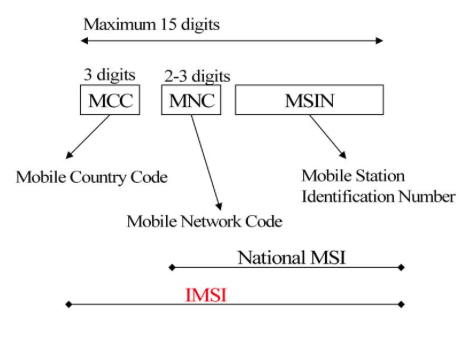
\includegraphics[width =  \linewidth]{./Pics/GSMITMSI} 
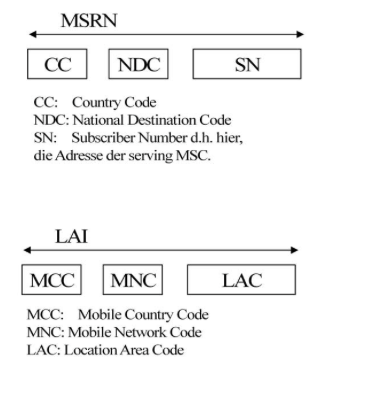
\includegraphics[width =  \linewidth]{./Pics/GSMMSRNUndLAI} 
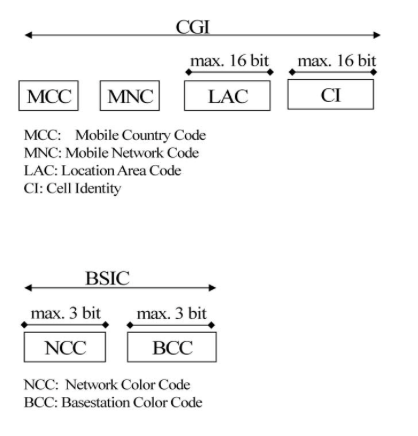
\includegraphics[width =  \linewidth]{./Pics/GSMCGIundBSIC} 
\end{minipage}

\subsection{Abläufe}
\subsubsection{Die Rolle der SIM}
Die SIM (Subscriber Identity Module) Karte ist die individuelle oder personalisierte Zugangsberechtigung zum PLMN.
\begin{itemize}
\item Die SIM Karte ist eine Chipkarte, die in eine MS eingefügt werden muss, um sich bei einem PLMN anzumelden
\item Die SIM speichert:
\begin{itemize}
\item Permanente Daten, z.B. IMSI, authentification key Ki, Liste der Trägerfrequenzen
\item Temporäre Daten, z.B. den aktuellen LAC, Zeitintervall für das location update, verbotene PLMNs....
\item Service-Daten, Service-Tabellen der zusätzlichen Dienstmerkmale, z.B. Spracheinstellungen, Taxiruf....
\end{itemize}
\item Es werden zwei Kartentypen unterschieden (gemäss Wikipedia 5)
\begin{itemize}
\item ID-1 SIM Card in Kreditkartengrösse (gemäss Wikipedia Standard SIM)
\item Plug-in SIM (kleiner als die ID-1) für semi-permanente Installation (gemäss Wikipedia Mini SIM)
\item seit 2003 Micro SIM, ist kleiner als Mini SIM (gemäss Wikipedia)
\item seit 2012 Nano SIM, ist kleiner als Micro SIM (gemäss Wikipedia)
\item in Zukunft Embedded SIM (gemäss Wikipedia)
\end{itemize}
\end{itemize}

\subsubsection{Sicherheitsprotokolle und die Rolle des AUC}

\begin{minipage}{0.5 \linewidth}
\begin{itemize}
\item Die Hauptaufgabe des AUC (Authentication Center) ist, die Informationen bereitzustellen, die das MSC/VLR benötigen um den Subscriber zu authentisieren und einen Schlüssel zur Verschlüsselung der Daten zu finden
\item Dazu erzeugt das AUC ein so genanntes Triplet
\begin{itemize}
\item RAND (Random Number)
\item SRES (Sigend Respons)
\item ein Schlüssel KC zur Verschlüsselung 
\end{itemize}
\item mit einer Anfrage werden 1,3 oder 5 Triplets erzeugt
\end{itemize}
\vspace{0.5 cm}
\textbf{Die Authentifizierung kann erfolgen bei}
\begin{itemize}
\item der Registrierung {attatching the Network}
\item jedem Verbindungsaufbau
\item jedem Location Updating
\item vor dem Start von Zusatzdiensten
\end{itemize}
\end{minipage}
\begin{minipage}{0.5 \linewidth}
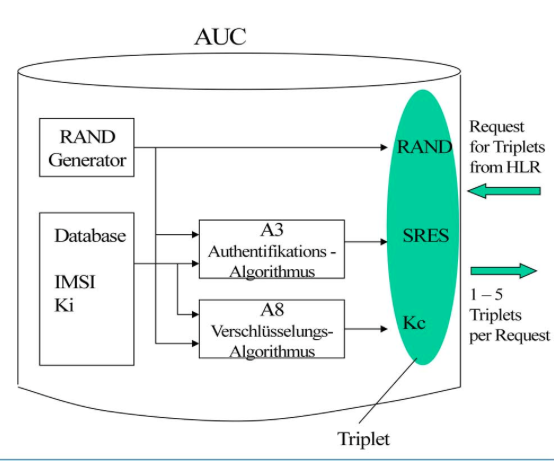
\includegraphics[width =  0.75 \linewidth]{./Pics/GSMAUC} 
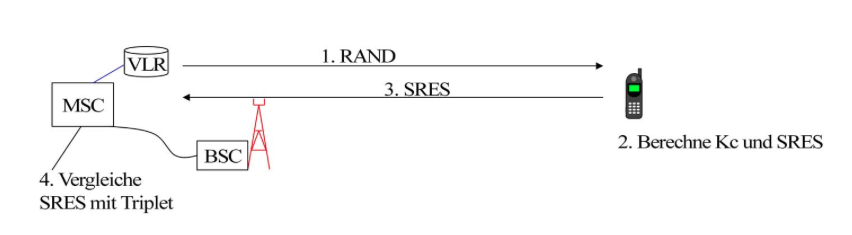
\includegraphics[width =  \linewidth]{./Pics/GSMAuthentifizierung} 
\end{minipage}
\subsubsection{Verschlüsselungsprozedur}
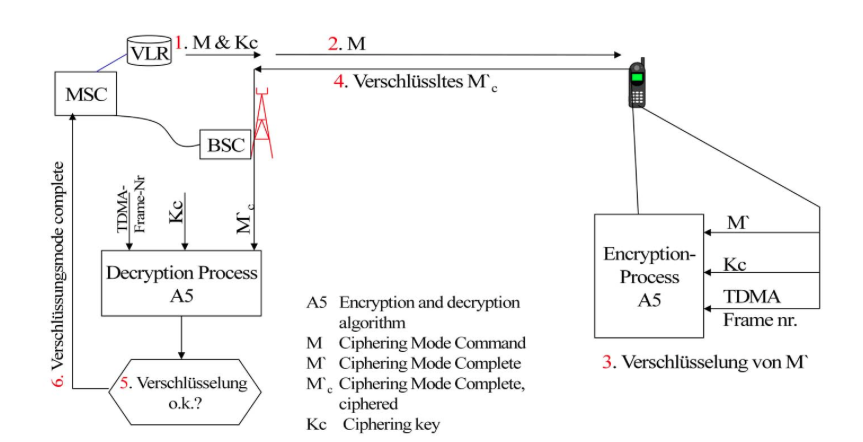
\includegraphics[width =  0.5 \linewidth]{./Pics/GSMVerschluesselung} 

\subsubsection{Anmeldeprozedur: IMSI Attach}
\begin{minipage}{0.5 \linewidth}
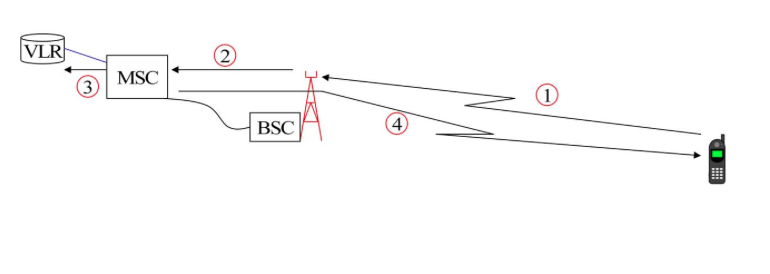
\includegraphics[width = \linewidth]{./Pics/GSMIMSIAttach}
\end{minipage}
\begin{minipage}{0.5 \linewidth}
\begin{enumerate}
\item Die MS sendet ein IMSI attach an das Netz mit der Zustandsangabe Idle.
\item Das VLR prüft, ob ein Datensatz der MS vorliegt. Liegt noch kein Datensatz vor, so kontaktiert das VLR das HLR und fordert die Subscriberinformation an. Hat sich ferner die LA geändert, so muss die neue LA ebenfalls ins VLR eingetragen werden
\item Das VLR setzt den Zustand der MS auf Idle
\item Es erfolgt eine Bestätigung an die MS, das die Anmeldung erfolgreich durchgeführt wurde.
\end{enumerate}
\end{minipage}

\subsubsection{Anmeldeprozedur: Location Update}
\begin{minipage}{0.5 \linewidth}
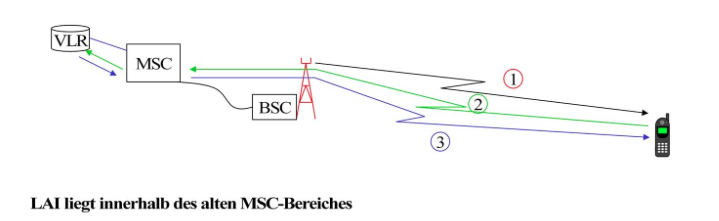
\includegraphics[width = \linewidth]{./Pics/GSMLocationUpdate}
\end{minipage}
\begin{minipage}{0.5 \linewidth}
\begin{enumerate}
\item Die MS hört ständig den aktuellen BCCH mit. Hier erhält sie unter anderem auch die Information über die LAI. Ist die LAI unterschiedlich der auf der SIM gespeicherten, so muss ein location update durchgeführt werden. 
\item Die MS muss dazu eine Verbindung zum Netz aufbauen (Anforderung eines SDCCH). Eine Authentisierung wird durchgeführt.
\item Ist die Authentisierung erfolgreich wird ein Location update Request an das System gesendet.
\item Hat kein MSC-Wechsel stattgefunden, so aktualisiert die aktuelle MSC den LAI im VLR und gibt den Signalisierungskanal wieder frei.
\end{enumerate}
\end{minipage}

\subsubsection{Abgehender Ruf}
\begin{minipage}{0.5 \linewidth}
\begin{enumerate}
\item Via RACH wird erst ein Signalisierungskanal angefordert
\item Die BSC teilt via AGCH der MS einen SDCCH zu
\item Die MS sendet eine set-up request an das MSC. Ferner werden die folgenden Prozeduren durchgeführt:
\begin{enumerate}
\item Die MS wird als aktiv im VLR eingetragen
\item Die Authentifizierungsprozedur wird durchgeführt
\item Die Verschlüsselung wird eingeschaltet
\item Die Ziel-Subscribernummer wird an das Netz übermittelt
\item Prüfen, ob abehender Rufe gesperrt sind
\end{enumerate}
\item Die MSC instruiert die BSC einen idle TCH zu reservieren. Ferner müssen sich die BTS und die MS auf den TCH synchronisieren
\item Die MSC leitet die Rufnummer weiter an die Zieladresse (ggf. PSTN)
\item Wenn der gerufene Teilnehmer antwortet werden die reservierten Kanäle geschaltet
\end{enumerate}
\end{minipage}
\begin{minipage}{0.5 \linewidth}
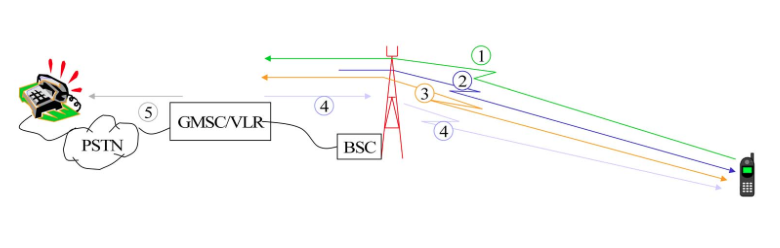
\includegraphics[width = \linewidth]{./Pics/GSMRuf}
\end{minipage}

\subsubsection{Ankommender Ruf}
\begin{minipage}{0.5 \linewidth}
Der Hauptunterschied zu einem abgehenden Ruf besteht darin, dass der Zielteilnehmer erst noch gesucht werden muss. Die MSISDN kann nicht unmittelbar für die Signalisierung genutzt werden. 

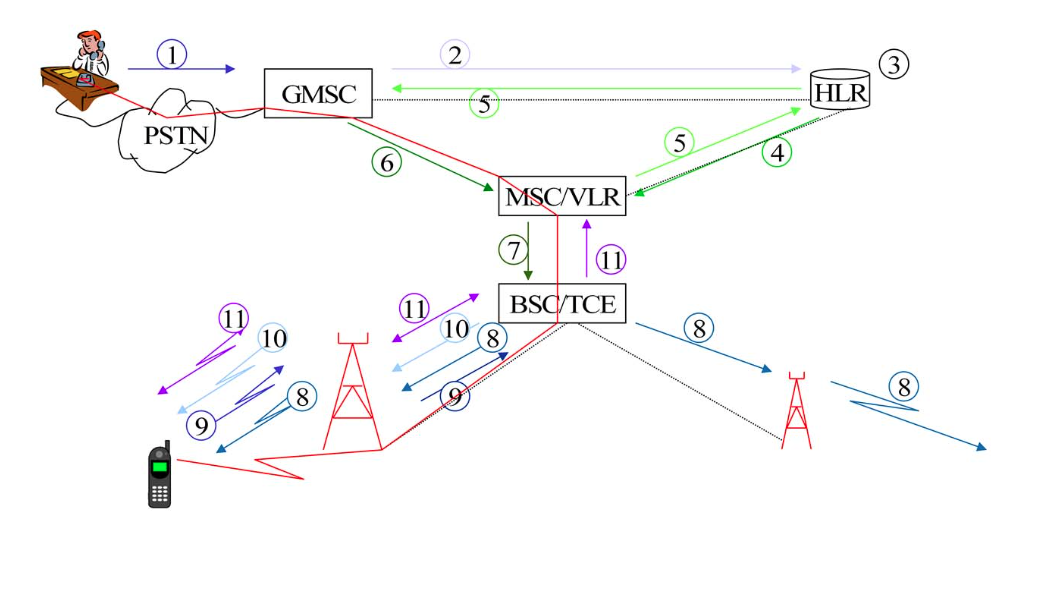
\includegraphics[width = \linewidth]{./Pics/GSMRuf2}
\end{minipage}
\begin{minipage}{0.5 \linewidth}
\begin{enumerate}
\item Die MSISDN wird im PSTN analysiert und an die GMSC weitergeleitet
\item Die GMSC des gerufen PLMN analysiert die MSISDN und fragt das HLR ab, zu welcher Serving MSC das Gespräch weitergeleitet werden muss. 
\item Das HLR überführt die MSISDN in die IMSI und entscheidet die Ziel MSC/VLR. Auserdem wird geprüft, ob zur Zeit Anrufe weitergeleitet werden sollen oder nicht
\item Das HLR fordert einen MSRN von der serving MSC/VLR an
\item Die serving MSC sendet via HLR die MSRN an die GMSC
\item Die GMSC wertet die MSRN aus und leitet den Ruf weiter
\item Die MSC/VLR kennt die LA und eine Paging-Nachricht wird an das BSC weitergeleitet
\item Die BSC leitet die Paging-Nachricht weiter an die BTSen der LA. Zur Identifikation dienen IMSI oder TMSI
\item Die MS antwortet mit einem request für einen SDCCH
\item Die BSC weist einen SDCCH über einen AGCH zu 
\item Die Call-set-up Prozedur wird durchgeführt und ein TCH reserviert sowie der SDCCH freigegeben
\item Die MS Signalisiert (ringing). Wird der Anruf angenommen wird durchgeschaltet
\end{enumerate}
\end{minipage}

\subsubsection{Handover}
\begin{minipage}{0.5 \linewidth}
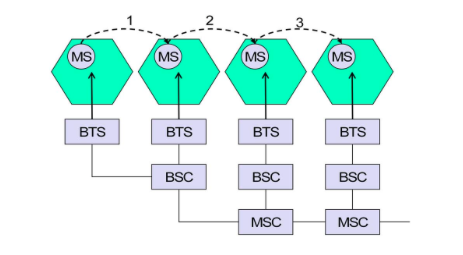
\includegraphics[width = \linewidth]{./Pics/GSMHandover}
\end{minipage}
\begin{minipage}{0.5 \linewidth}
\begin{enumerate}
\item Intra BSC Handover. BSC ist involviert.
\item BSC/Intra MSC Handover. Die BSC wird gewechselt. MSC ist involviert.
\item Inter MSC Handover. MSC wird gewechselt. Die alte MSC wird anchor MSC genannt, die neue MSC dann serving MSC nachdem der Handover abgeschossen ist. Das Billing (Verrechnung) wird jedoch immer von der anchor MSC gemacht. Das bedeutet, dass der Traffic immer von der serving MSC zur anchor MSC (uplink) und von der anchor MSC zur serving MSC (downlink) geleitet wird.
\end{enumerate}
\end{minipage}
\begin{minipage}{0.5 \linewidth}
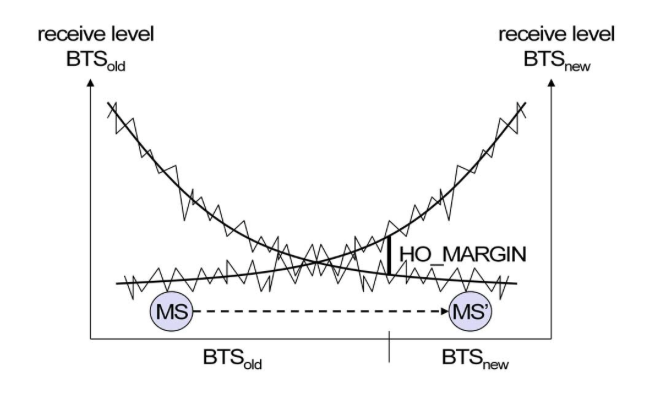
\includegraphics[width = \linewidth]{./Pics/GSMHandover2}
\end{minipage}
\begin{minipage}{0.5 \linewidth}
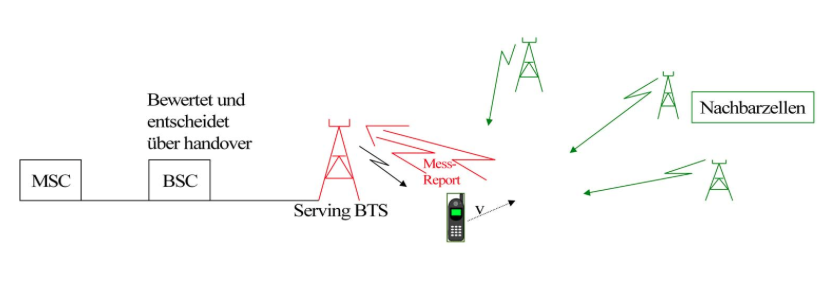
\includegraphics[width = \linewidth]{./Pics/GSMHandover3}
\end{minipage}

\begin{minipage}{0.5 \linewidth}
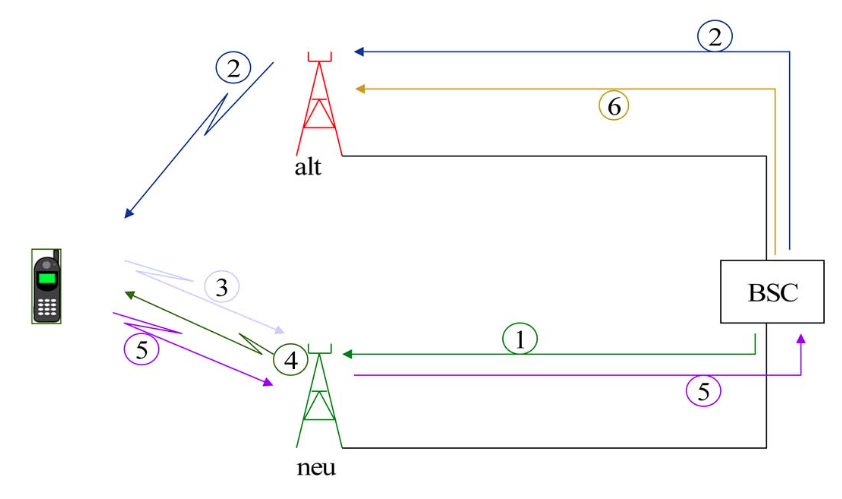
\includegraphics[width = \linewidth]{./Pics/GSMIntraHO}
\end{minipage}
\begin{minipage}{0.5 \linewidth}
\begin{enumerate}
\item Die BSC reserviert einen TCH in der neuen BTS
\item Die MS wird über die alte Verbindung (FACCH) über die neue Frequenz, den Time Slot und die Sendeleistung informiert
\item Die MS synchronisiert auf die Frequenz, die Rahmenstruktur und überträgt einen Handover Request über den FACCH. Der Handover Request hat nur einen Grösse von 8 Bit
\item Die BTS sendet die TA Information via FACCH
\item Die MS sendet ein Handover complete zur BSC über die neue BTS
\item Die alte BTS wird aufgefordert den TCH freizugeben, die Verbindung wird durchgeschaltet
\end{enumerate}
\end{minipage}

\begin{minipage}{0.5 \linewidth}
\begin{enumerate}
\item Die serving BSC sendet ein Handover Request an die MSC/VLR mit der ID der Zielzelle
\item Die MSC/VLR identifiziert die neue BSC und sendet ein Handover Request an die neue BSC
\item Die neue BSC reserviert einen TCH
\item Die BSC sendet eine Message via MSC und alte BSC an die MS
\item MS synchronisiert mit der neuen Frequenz auf neuem Timeslot und sendet Handover Request
\item Information über die TA wird übertragen
\item Die MS sendet Handover complete
\item Die MS sendet der alten BSC die Aufforderung den alten TCH freizugeben
\item Der alte TCH wird freigegeben. Die Verbindung ist durchgeschaltet 
\end{enumerate}
\end{minipage}
\begin{minipage}{0.5 \linewidth}
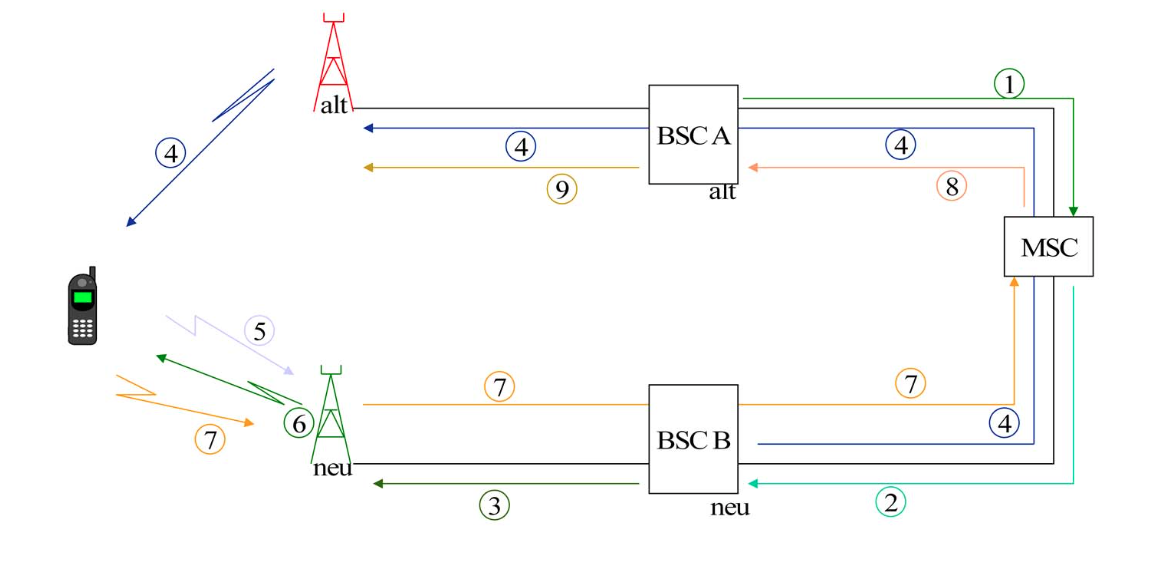
\includegraphics[width = \linewidth]{./Pics/GSMInterHO}
\end{minipage}

\begin{minipage}{0.5 \linewidth}
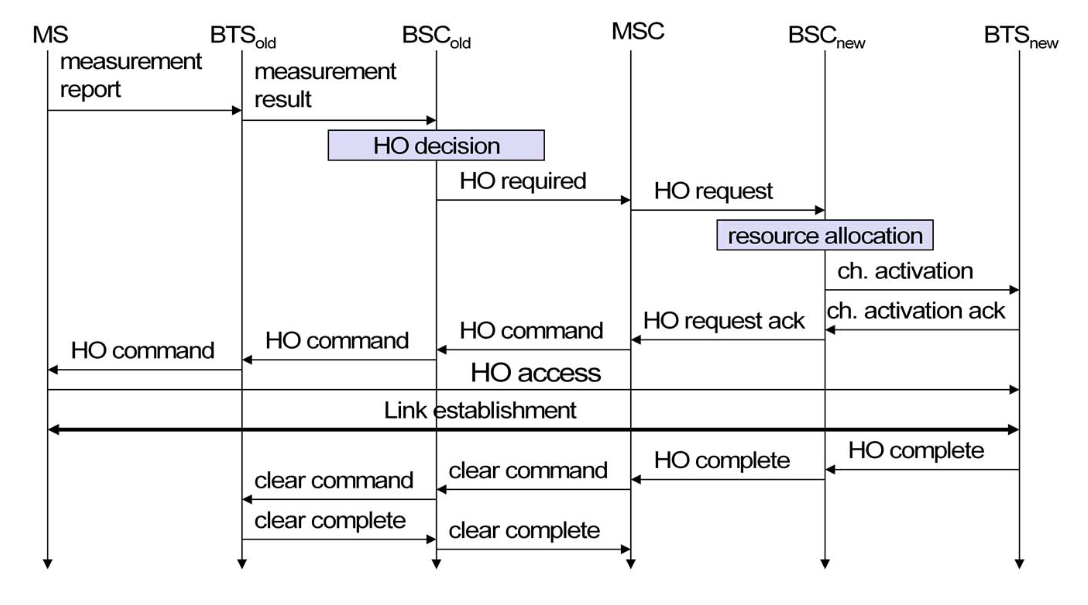
\includegraphics[width = \linewidth]{./Pics/GSMInterMSCHO}
\end{minipage}
\begin{minipage}{0.5 \linewidth}
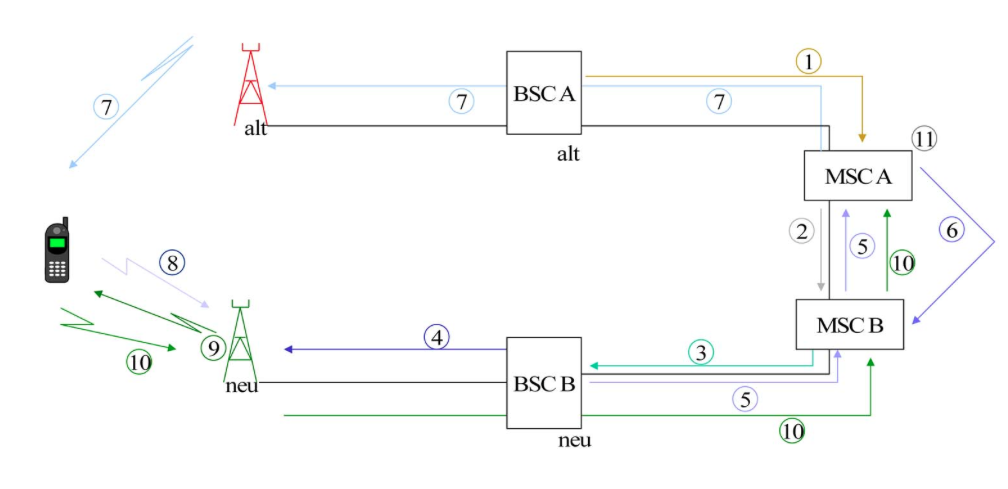
\includegraphics[width = \linewidth]{./Pics/GSMInterMSCHO2}
\end{minipage}

\begin{enumerate}
\item Die serving BSC sendet ein Handover Request an die MSC/VLR mit der ID der Zielzelle
\item Die MSC/VLR identifiziert die neue Zelle in einer anderen MSC und sendet ein help request an die neue MSC
\item Die neue MSC alloziert eine Handover-Number um den Ruf neu zu schalten. Ein Handover Request wird an die neue BSC gesendet
\item Die neue BSC reserviert einen TCH in der neuen Zelle
\item Die neuen BSC sendet eine Message (Zellinfo und Handover-Nummer) via MSCs und alte BSC an die MS
\item Es wird eine Verbindung zur neuen MSC geschaltet
\item Die MSC A sendet das Handover Command an die MS
\item Ms synchronisiert mit der neuen Frequenz auf neuem Timeslot und sendet Handover Request 
\item Information über die TA wird übertragen
\item Die MS sendet Handover Complete
\item Ein neuer Weg wird in der aletn MSC geschaltet und die Verbindung wird geschaltet
\item Die MSC sendet der alten BSC die Aufforderung den alten TCH freizugeben (nicht mehr im Bild eingetragen). Die Verbindung ist durchgeschaltet. 
\end{enumerate}
Die alte Msc behält die Hauptkontrolle über die Verbindung, bis sie ausgelöst wird.

\subsubsection{Roaming}
\begin{itemize}
\item Der prinzipielle Ablauf ist dem Anmelden im eigenen Netz identisch
\item Erst versucht die MS sich im eigenen Netz anzumelden, ist dies nicht möglich sucht es andere BCCH-Träger von fremden Netzen
\item Dann vergleicht es die gefundenen Netzte mit der Liste der verbotenen PLMNs (Auf SIM gespeichert)
\item Findet die MS ein geeignetes Netz, so läuft die Anmeldeprozedur wie vorher besprochen, nur dass das HLR des eigenen Netzes konsultiert wird
\end{itemize}

\subsubsection{HSCSD - High Speed Circuit Switched Data}
\begin{itemize}
\item Herkömmlich Datenübertragung ist standardisiert mit 9.6 kbit/s
\begin{itemize}
\item Gesicherte Datenübertragung geht runter bis auf 4.8 kbit/s
\item So genanntes advanced coding erlaubt 14.4 kbit/s
\end{itemize}
HSCSD High Speed Circuit Switched Data
\begin{itemize}
\item ist standardisiert
\item Bündelung von bis zu 4 TDMA-Slots, um eine höhere Datenrate zu erreichen. (AIUR Air Interface User Rate)
\item Vorteile:
\begin{itemize}
\item Verfügbar
\item Konstante Qualität
\item Einfach
\end{itemize}
\item Nachteile:
\begin{itemize}
\item Kanäle blockiert
\item Teuer für den Benutzer
\end{itemize}
\end{itemize}
\end{itemize}


\subsection{GPRS - General Packet Radio Service}
\subsubsection{Überblick}
\begin{itemize}
\item Datnepaket-Dienst
\item Dynamische Bündelung freier Slots zu hochbitratigen Datenkanälen, je nach coding Schema 8 bis 21.4 kbit/s
\item asymetrische Übertragung - Slots werden nur belegt, wenn effektiv übertragen wird
\item Gebühren nach Datenmenge und nicht mehr nach Zeit
\item Standartisierung 1998, Einführung 2001/2002
\item Erweiterung der bisherigen Netztopologie
\item geplant ist ein komplementärer Einsatz von GSM/GPRS und UMTS
\item Harmonisierung Internet und Mobilnetz dank IP
\end{itemize}
\subsubsection{GPRS Netzelemente}
\begin{itemize}
\item GSN: GPRS Support Nodes
\begin{itemize}
\item GGSN Gateway GSN - Gateway zu PDNs(Public Data Network)
\item SGSN Serving GSN - unterstützt die MS(location, billing security)
\end{itemize}
\item GR: GPRS Register - eine Ergänzung zum HLR zur Adressverwaltung
\item PCU Packet Control Unit - Übernimmt BSC Funktion im paketorientierten Netzwerk
\end{itemize}

\subsubsection{Architektur Übersicht}
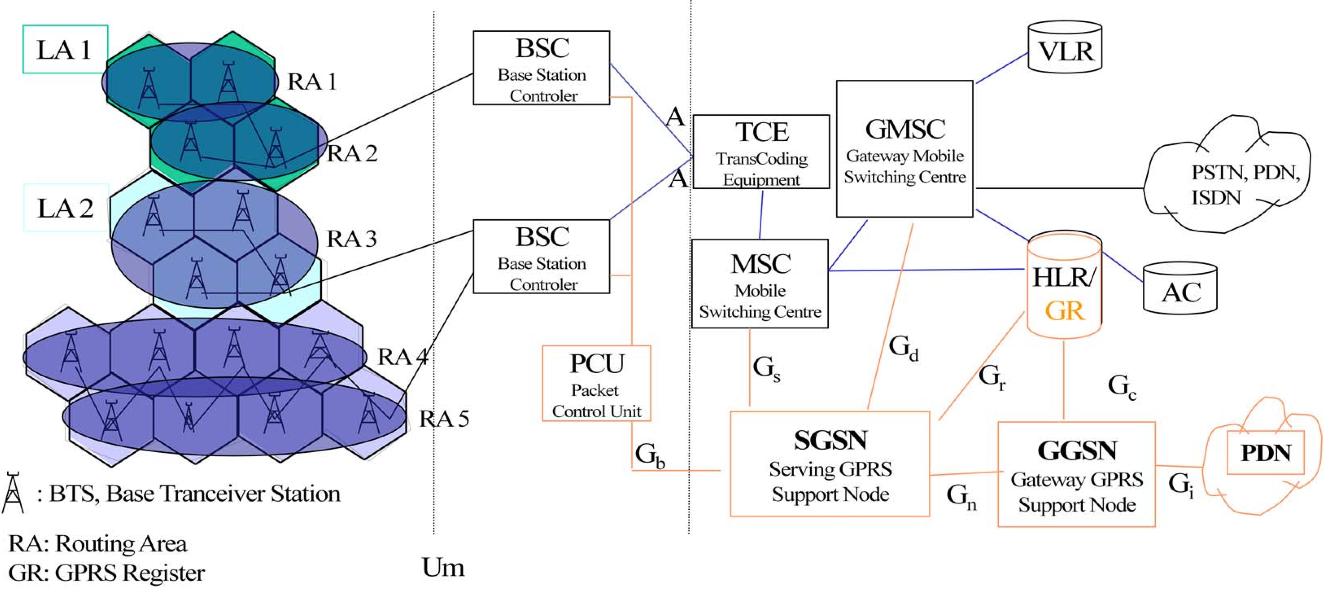
\includegraphics[width = \linewidth]{./Pics/GPRS.png} \\
Diese Grafik zeigt sehr gut, dass das GPRS kein neues Netz ist sondern eine Erweiterung von GSM. Orange eingefärbt sieht man die neuen Element. Man hat nun neben dem Verbindungsorientierten GSM Netz noch ein Paketorierntiertes GPRS Datennetz. Dieses Netz wird ausschliesslich zur Datenübertragung verwendet und kann wegen einer sehr hohen latenzzeit (bis 500ms) auch nicht für VOIP verwendet werden.

\subsubsection{Protocol stack}
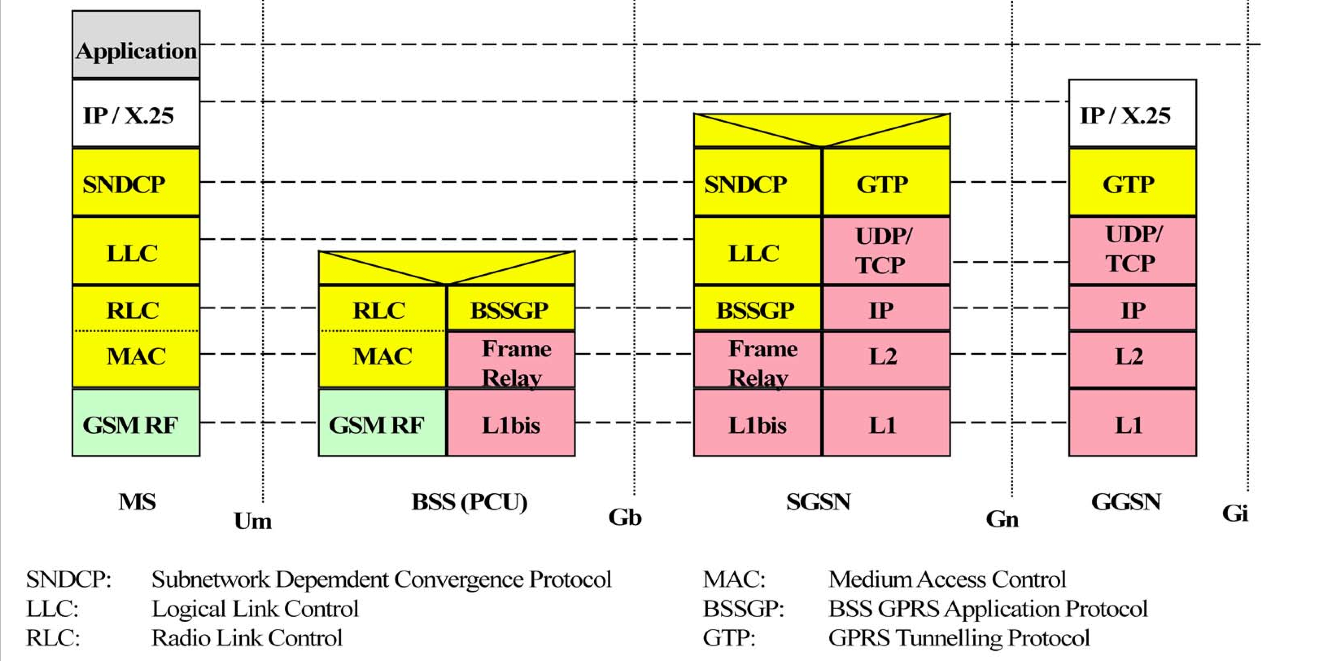
\includegraphics[width = \linewidth]{./Pics/GPRS2.png}

\begin{tabular}{|l|l|l|l|}
\hline
IP & Internet Protocol & X.25 & vorläufer von IP \\
SNDCP & Subnetwork Dependent Convergence Protocol & LLC & Logical Link Control \\
RLC  & Radio Link Control  & MAC & Medium Access Control \\
GSM RF &  Global System for Mobile Communications Radio Frequencies & BSSGP & Base Station System GPRS Protocol \\
GTP & GPRS Tunnelling Protocol & UDP & User Datagram Protocol \\
TCP & Transmission Control Protocol & & \\ 
\hline
\end{tabular}
\subsubsection{GTP}
Das GPRS Tunnelling Protocol baut IP-basierte Verbindungen durch den Backbone auf. Datenpakete werden eingepackt \& unter Benutzung des GTP getunnelt. GTP nutzt unterhalb TCP oder UDP  abhängig von der Nutzeranforderung. Das ganze GPRS Netzwerk basiert auf einem IP Hop, was das Routing im Backbone bei Mobilität vereinfacht.



\subsection{MPS - Mobile Positioning System}

\subsubsection{Verwendung}
\begin{description}
\item [MPS] Mobil Position Services
\item [Legal interception] Verfolgung von und Zugriff auf Zielpersonen durch die Polizei
\item [Desaster and Emergency Management] Suche nach vermissten und/oder hilflosen Personen
\end{description}
\vspace{0.5cm}

\begin{itemize}
\item Forderung durch Standards
\begin{itemize}
\item NG911(Next Generator 911): Suchradius < 10 m in 95 \% der Suchfälle
\end{itemize}
\item Hauptproblem
\begin{itemize}
\item Unterscheidung Nah- und Fernbereich
\item In Urbanen Regionen mit Häuserschluchten (Abdeckungen/Reflexionen)
\end{itemize}
\end{itemize}

\subsubsection{Verfahren zur Positionsbestimmung: Überblick}

\begin{minipage}{0.7 \linewidth}
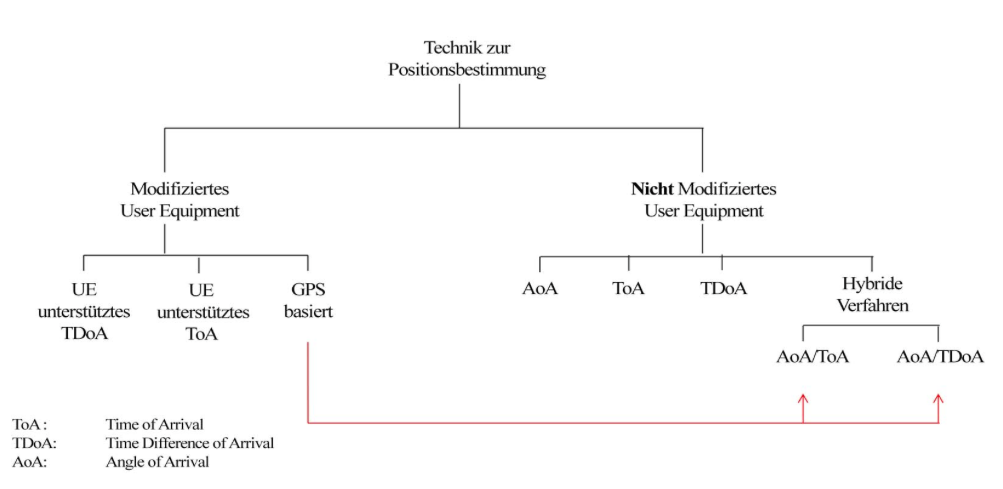
\includegraphics[width =\linewidth]{./Pics/MPS}
\end{minipage}
\begin{minipage}{0.3 \linewidth}
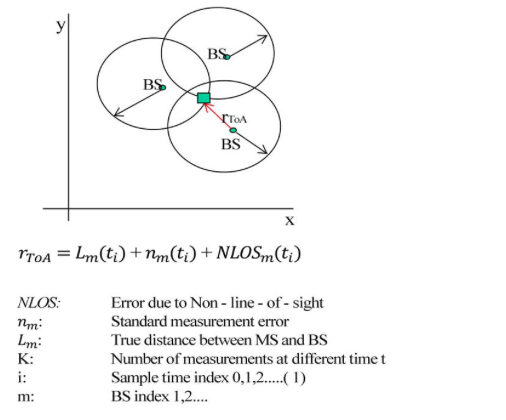
\includegraphics[width = \linewidth]{./Pics/TDoA}
\end{minipage}

TDoA oder hyperbolig PL Technique ist eine Verfeinerung der ToA und basiert auf einer zeitsynchronisierten (GPS) Location Measurement Units (LMUs) der Base Station.

Die LMUs wertet jeden UPLinkCall eines Subscribers aus. 

Das heute implementierte System bringt eine Genauigkeit kleiner 50m, benötigt werden aber eine freie Sicht zu mindestens 3 BS, je mehr desto besser. 

\subsubsection{Gegenstand der Forschung}
\begin{itemize}
\item Kombination von Mobilnetz und anderen RF Systemen Wi-Fi
\item Fehler Optimierung der ToA/TDoA Technologien
\item AoA Techniken, Probleme der Winkelbestimmung, Herausforderung an die Elektrotechnik - Antennen mit synthetischer Apertur
\item Phasenanalyse des Trägers, Probleme bei langsamen Mobilstationen (kein Dopplereffekt)
\item Auswertung typischer Netzwerkeigenschaften
\begin{itemize}
\item Messreports, Cell ID, Signal Fingerprints
\item Nachteil: der provider muss Daten vorhalten
\end{itemize}
\item Kombination von GPS(Empfang von nur einem Satelliten zur Zeitsynchronisation) mit ToA Phasenanalyse
\end{itemize}